\chapter{Structured Characters}
This chapter presents a concept to embed structured data in an atomic character. It is used to enable data structures, like \code{EObjects} on the character input stream for the lexer. The general idea is to use private characters as keys for a map. These special characters, which identify an object are called ``ID Characters'' in the following.

\section{General Requirements}
The task of an ID Character is to uniquely identify an object in a serializeable context. 
The ideal characteristics are:
\begin{itemize}
	\item bindable and existence depedant on another character or standalone
	\item unlimited number of unique identifiers
	\item atomic. The integritiy should be perserved and not be unbreakable.
	\item standardised. There should be a long term guarantee that their are available for use.
	\item ubiqious available. They should be available on every platform.
	\item abstract characters. They should be fast distinguisable from non ID character
	\item private. They should not causes any conflicts or be missinterpretable in any way.
\end{itemize}

\subsection{Unicode Private-Use Characters}
A possible solution offers Unicode \cite{Unicode}. Unicode is a universal character encoding standard for consistent encoding and exchange of text data. It is the default encoding of HTML and XML and is implemented in all modern operating systems. It specifies a numeric value (code point) and name for each character. Unicode was developed in conjunction with the Universal Character Set and can be represented by widely available encodings like UTF-8. The Unicode Standard defines private-use characters, which interpretation is not specified and is determined by a private agreement among cooperative users. For example Apple uses a private character to present it's apple logo. A application specific changed interpretation of for example the character representing the apple logo is valid, as it specifies its intended behaviour according to a private agreement.\\
The private use characters are intended for softwaredevelopers. They can be compared to the ideal characteristics:
\begin{itemize}
	\item they are stand alone characters and are not bindable per se.
	\item The number of identifiers is limited to 137,468, in which 6,400 are in the private use area U+E000 to U+F8FF and 65,534 are in each supplementary private use Area-A and Area-B. 
	\item They are single characters and thus atomic. 
	\item Unicode is standardised and private-use characters are permanently designated for private use.
	\item Unicode, especially the UTF-8 enconding is wide spread and nearly ubiqious avaiable on modern personal computer platforms.
	\item There are three code-blocks for private-use characters. Three range check for a code point is in sufficient to determine its private-use.
	\item Private-use characters are, as the name states, explicitly designed for private use.
\end{itemize}

The restriction of a limited number of available identifiers could be solved by implementing a non-standard character encoding, probably a variable-with enconding.

\section{Use and implementation of the ID-Character}
The possible use of an ID character is twofold:
\begin{itemize}
	\item adding an ID to a character
	\item using the ID to refer an EObject
\end{itemize}
To extend the use of an ID character, it could be extended with an associatitivy: right, none or left.
It is therefore mandatory to save this addional information in an associated resource. The above restriction to an EObject ensures XMI serializablitiy. The resource should contain a map from ID character to a triple containing the associativity, the ID or UUID and an EObject). The associativity determines if it's a plain ID or as a reference character. Non associative characters are EObject references. The second place can't be shared in case the extrensic UUID of the EObject should be preserved.

ID characters could be implemented by wrapping the existent lexical analyser. The wrapping lexer loads the additional resource and resolves the ID if it is found on the input strema. If a non associative ID character is resolved and regular the next character of the normal lexer is after the ID character, it is cached and the resolved ID character is returned. In case the current position on the character stream is not smaller than the positition of the ID character, the character of the regular parser is returned. In case of plain ID characters with right associativtiy the ID is assigned to a property of the character return by the wrapped lexer. Left associative characters require a lookahead of one regular character and should be avoided for this reason. Also, in the case the wrapping parser doesn't know about the ignored characters, this requires that it inspects the returned normal character to recongnize errors where an ID character was contained in a regular character. The primary use of an ID character is likely to let the lexer return an EObject to the parser as an atomic character.

\begin{figure}
\centering
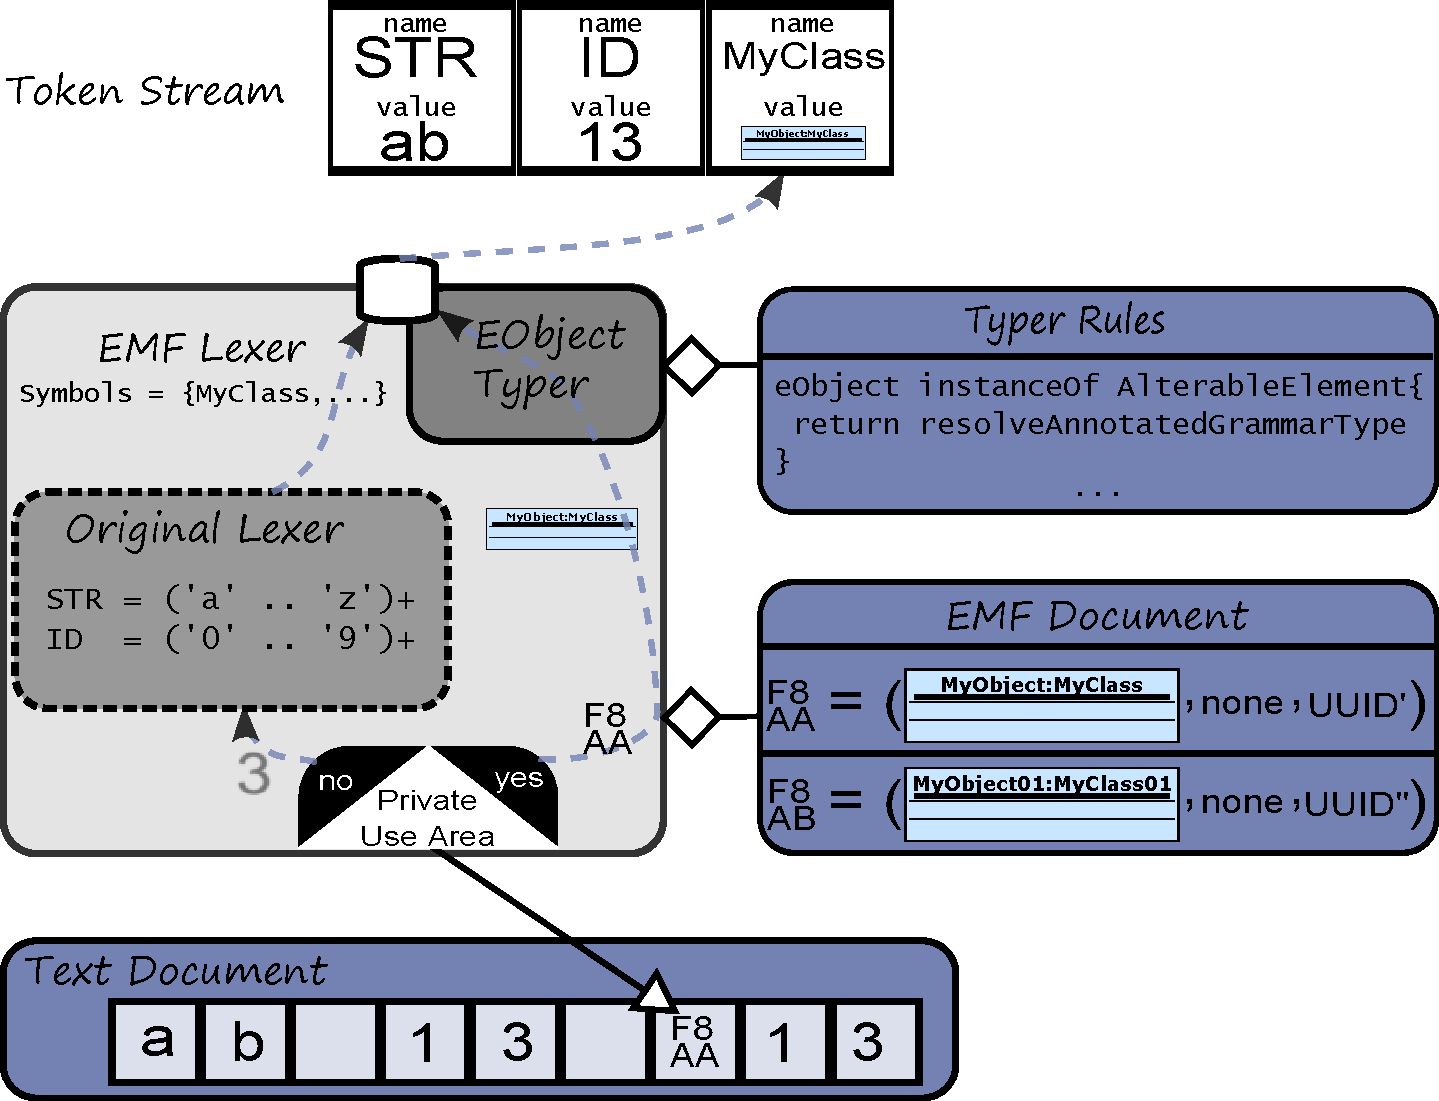
\includegraphics[scale=0.55]{gfx/ex/Lexer} 
\caption{EMF Lexer extension}
%\label{MM:GrammarUML}
\end{figure}


\section{Use cases}
The definition of ID characters, unparser and notation model don't in the previous sections just indicated their amended use. This sections describes their intergrated use and how the concepts leaverage each other. \todo{review the need of ID character handling by the editor, play scenarios to gain pages?}

\subsection{Incomplete information handling}
The first, obvious benefit of ID characters is that the textual representation doesn't nessessarly need to describe the whole model. It enables the use of EObject directly in the grammar and thus the grammar to properly handle parts of the lanuage. The results in inablity to modify the unhandeled parts and the existence of an ID character, or a character placeholder at the unhandeled location. This shifts the problem of handling this ID character to the text editor.

\subsection{Different representations of semantic equivalent tokens}
In case the unparser found more than one valid grammar rule for a notation element, the corresponding transient field is set. The text editor should offer the user the change the current representation value, which reassigns the grammar rule of the current notation element and, if necessary, also to its decendants. As soon as the reassignment is finished, a new token stream is produced reflecting the new textual representation.


\subsection{Sententential Tokens \& Graphical Editors}
Because the notation model is the parse and consists of EObjects, it is possible to serialize notation nodes as single ID tokens. Sentential tokens are tokens which represent a sentenential production. The additional definition of sentential tokens circumvents the contradicting statement of nonterminal tokens on the input token stream. This concept is necessary for incremental parsers and can be leaveraged for visual editing. This can be used to fold parts of the word into an ID token. This ID token is completely grammar conform. The main benefit is not folding of word parts but to allow a graphical editor to be presented at the ID tokens location editing the refered language object. It is important to mention, that the editor edits a language object, but is a substitute or semantic equivalent of a specific terminal or nonterminal, or a set, but never a sequence of them. This means that the editor may edit the language object and its descendants just as long as the unparser allows one of the editors semantic equivalents at the current position. If the graphical editor nests textual representation, it must create an own parser instance. This parser instance can be of the same type as the outer parser instance with a different start symbol, but doesn't has to be. It must be sychronized to the same language model. It might also reuse the noation model, which is guaranteed if a new instance of the outer parser is used.

\todo{each notation model element as stateless edit part} \\
\todo{annotation special} \\
\todo {sententential tokens as generated grammar productions} \\